\section{Diseño eléctrico}

En esta sección se muestran los distintos elementos del desarrollo en el plano eléctrico y electrónico.

\subsection{Diagrama eléctrico}

La Figura \ref{de_diagrama} muestra el diagrama eléctrico principal, este cuenta con los siguientes elementos:
\begin{itemize}
    \item \textbf{Batería}: La batería corresponde a un pack de 4 celdas de polímero de litio. Posee un voltaje nominal de \SI{14.8}{\volt} y una capacidad de \SI{3300}{\milli\ampere\hour}. Este tipo de baterías se caracterizan por su gran densidad energética y capacidad de descarga, por lo es óptima para la operación de motores, pues usualmente requieren peaks corriente del orden de \SI{5}{\ampere}.
    \item \textbf{Panel de control}: En su interior contiene el microcontrolador y receptor de radio.
    \item \textbf{Interruptor principal}: Es el encargado de conectar la batería con el resto de los circuitos.
    \item \textbf{Interruptor de emergencia}: Desconecta la energía del bus de actuadores Dynamixel, no interfiere con la alimentación del panel de control.
    \item \textbf{Bus Dynamixel}: Este bus esta constituido por cuatro conductores. Dos de ellos proporcionan alimentación a los dispositivos conectados ($V_{cc}$ y tierra). Los otros dos corresponden a la señal diferencial del bus RS485.
\end{itemize}

\begin{figure}[H]
\begin{center}
	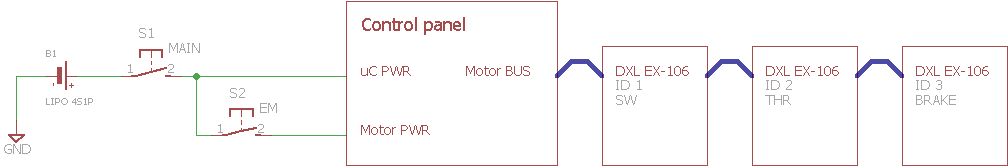
\includegraphics[width=0.9\textwidth]{diseno_electrico/diagram.png}
	\caption{Diagrama elétrico principal.}
	\label{de_diagrama}
\end{center}
\end{figure}

\subsection{Sistema de radio}

Para la comunicación con el GoKart a través de telecomandos se está utilizando un transmisor de radiofrecuencias llamado Fly-Sky modelo FS-T6, junto a un receptor de 6 canales a 2.4 GHz llamado Fly-Sky modelo FS-R6B (ver en Figura \ref{rf}).

\begin{figure}[H]
    \centering
    \begin{subfigure}[b]{0.3\textwidth}
        \centering
        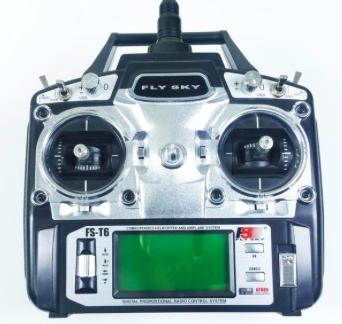
\includegraphics[width=0.9\textwidth]{diseno_electrico/rf_control.png}
        \caption{Control remoto}
        \label{rf_control}
    \end{subfigure}
    \begin{subfigure}[b]{0.3\textwidth}
        \centering
        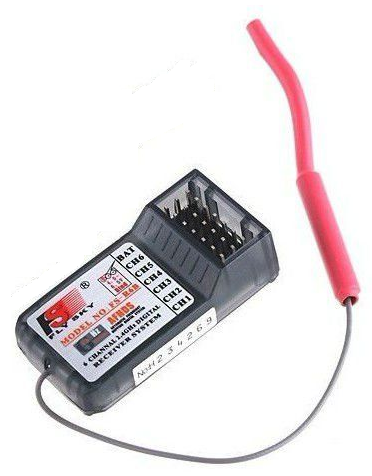
\includegraphics[width=0.9\textwidth]{diseno_electrico/rf.png}
	    \caption{Receptor de radio}
	    \label{rf_img}
    \end{subfigure}
    \caption{Hardware utilizado para telecomandar el gokart}\label{rf}
\end{figure}

De la radio transmisora se utilizarán 3 comandos:
\begin{enumerate}
    \item {\textbf{Manilla izquierda:} movimientos UP y DOWN para acelerar y frenar, respectivamente.}
    \item {\textbf{Manilla derecha: } movimientos LEFT y RIGHT para dirección.}
    \item {\textbf{Switch superior izquierda:} para activar estado de emergencia. }
\end{enumerate}

De esta forma, el receptor utiliza 3 de sus 6 canales para recibir los datos, los que resultan ser números enteros con un rango entre 1000-1400, que corresponden al valor en \si{\micro\second} del up-time de la señal PWM recibida.

\subsection{Sistema embebido}

El sistema cuenta con un microcontrolador principal encargado de recibir los comandos desde el receptor de radio y enviar comandos de movimiento a los servomotores. El sistema usa como elemento principal una placa de desarrollo Arduino Mega 2560 \cite{arduino_mega}, que se muestra en la Figura \ref{arduino_mega_img}. La Tabla \ref{arduino_mega_tab} muestra las principales características de la placa de desarrollo.

\begin{table}[H]
\centering
\begin{tabular}{|l|l|}
\hline
Microcontrolador        & ATmega2560                              \\ \hline
Voltaje de operación    & \SI{5}{\volt}                           \\ \hline
Limites de alimentación & \SI{6}{\volt} a \SI{20}{\volt}          \\ \hline
GPIO                    & 54                                      \\ \hline
Entradas ADC            & 16                                      \\ \hline
Memoria Flash           & \SI{256}{\kilo\byte}                    \\ \hline
SRAM                    & \SI{8}{\kilo\byte}                      \\ \hline
Velocidad de reloj      & \SI{16}{\mega\hertz}                    \\ \hline
Puertos UART            & 4                                       \\ \hline
\end{tabular}
\caption{Características Arduino Mega 2560}
\label{arduino_mega_tab}
\end{table}

\begin{figure}[H]
\begin{center}
	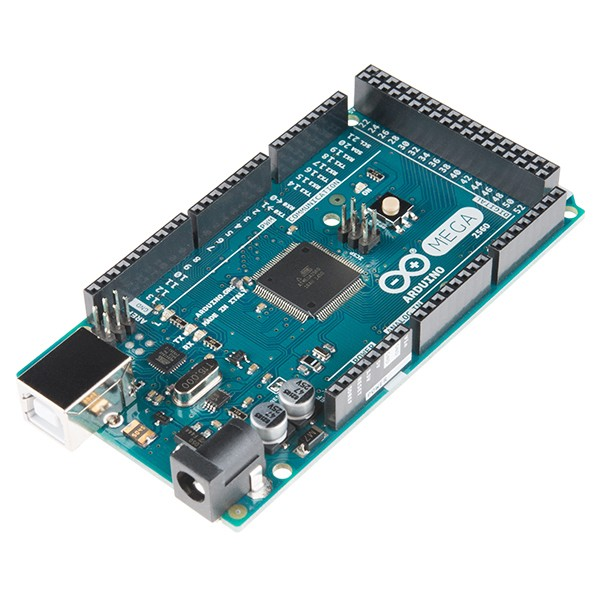
\includegraphics[width=0.3\textwidth]{diseno_electrico/arduino-mega.jpg}
	\caption{Arduino Mega 2560.}
	\label{arduino_mega_img}
\end{center}
\end{figure}

\subsubsection{Pantalla LCD}

La pantalla LCD empleada corresponde a LCD \textit{keypad shield} \cite{arduino_lcd}, esta placa es compatible con el extendido controlador Hitachi HD44780. La Figura \ref{arduino_lcd} muestra la placa utilizada.

\begin{figure}[H]
\begin{center}
	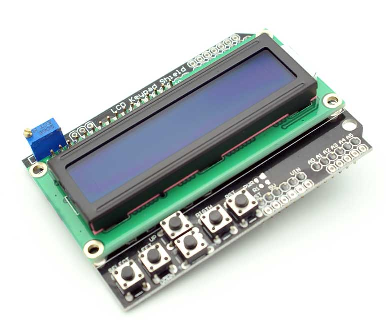
\includegraphics[width=0.5\textwidth]{diseno_electrico/lcd.png}
	\caption{LCD \textit{keypad shield} utilizado.}
	\label{arduino_lcd}
\end{center}
\end{figure}

\subsubsection{Interfaz con motores Dynamixel}

Los actuadores utilizados en este proyecto corresponden al modelo Dynamixel EX-106+ fabricados por Robotis. Estos actuadores son ampliamente utilizados en aplicaciones robóticas, integran su propio controlador, encoder, driver e interfaz de comunicación que permite la conexión de múltiples actuadores usando como capa física un bus RS485.

Para la conversión del puerto UART del del microcontrolador al estándar RS485 es necesario un \textit{transceiver}, en está aplicación se uso un integrado SN75176BP de Texas Instruments \cite{ic_rs485}.

Para la comunicación con los actuadores Dynamixel es necesario usar un protocolo especificado por el fabricante \cite{motor_datasheet}, dado la gran extensión de estos motores existen librerías que proveen una interfaz de software que implementan el protocolo.

\subsubsection{PCB}

Para el montaje del receptor de radio y componentes necesarios para la comunicación con los motores Dynamixel, se diseñó y construyó una PCB que se se empotra de forma natural a la placa Arduino Mega, pues se ha usado el formato conocido como \textit{shield}.

La Figura \ref{de_pcb} muestra el diseño de la PCB, donde se ha considerado las conexiones para el \textit{transceiver} RS485, una pantalla LCD y potenciómetros para hacer una interfaz de usuario.

\begin{figure}[H]
\begin{center}
	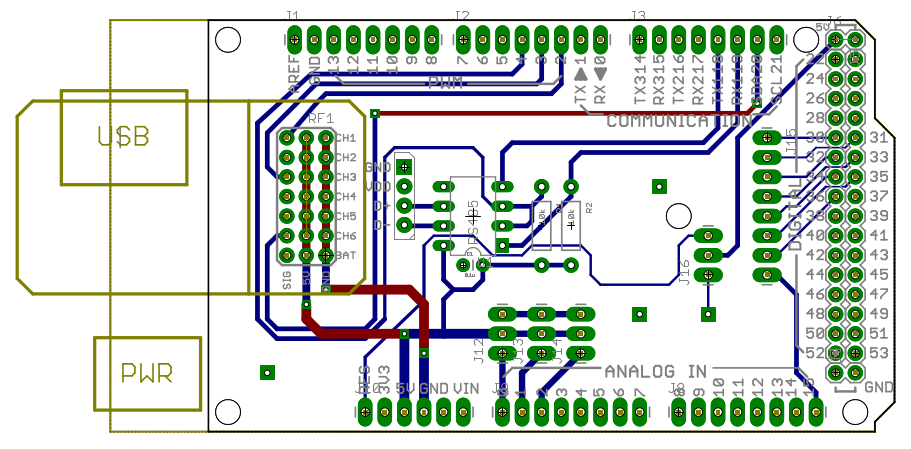
\includegraphics[width=0.5\textwidth]{diseno_electrico/pcb.png}
	\caption{PCB con formato \textit{shield}.}
	\label{de_pcb}
\end{center}
\end{figure}



